\chapter{Results \& Discussion}

\section{Validation}
Variables are determined in the previous section. In this section, by using these variables and the model, five different plots regarding the different set temperatures and trials are generated to compare the model's results with the experimental data. 
\par
Validation plots are provided below in Figures \ref{fig:test3}, \ref{fig:test4}, \ref{fig:test5}, \ref{fig:test6} and \ref{fig:test7}.

\begin{figure}[h]
    \begin{minipage}{.5\textwidth}
        \centering
        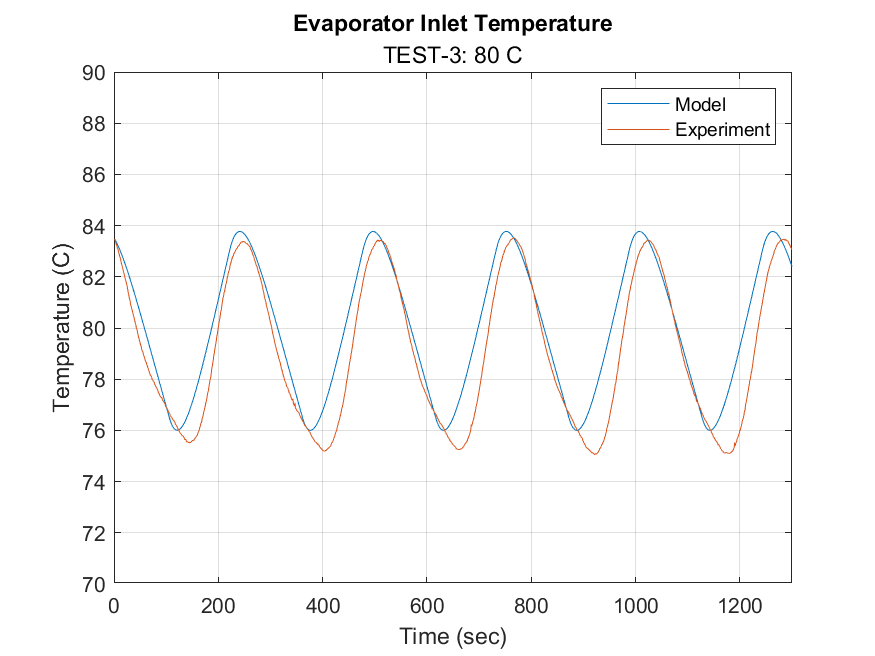
\includegraphics[width=8cm]{images/TEST-3.png}
        \captionof{figure}{Test-3.}
        \label{fig:test3}
    \end{minipage}
    \begin{minipage}{.4\textwidth}
        \centering
        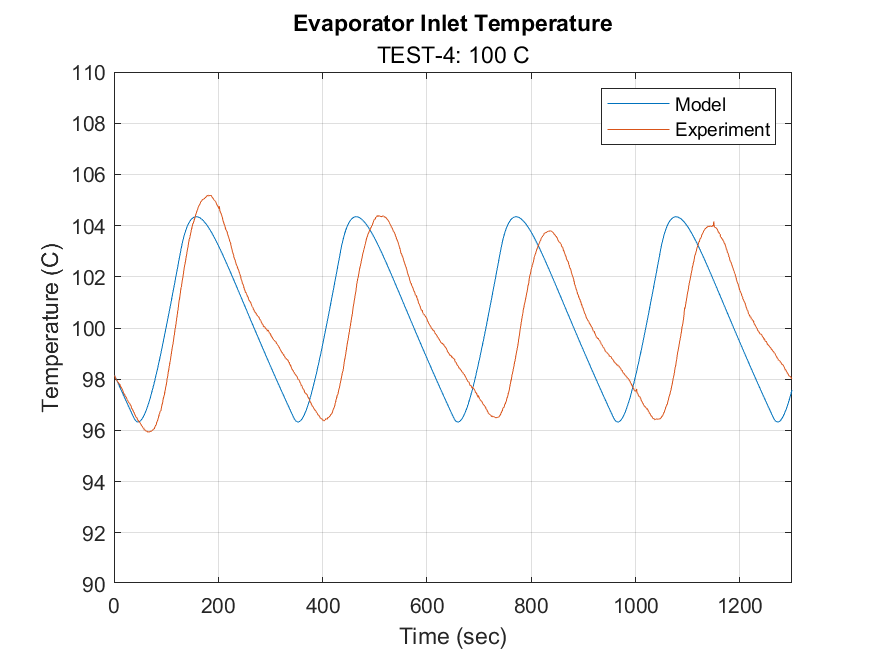
\includegraphics[width=8cm]{images/TEST-4.png}
        \captionof{figure}{Test-4.}
        \label{fig:test4}
    \end{minipage}
\end{figure}

\bigskip

\begin{figure}[h]
    \begin{minipage}{.5\textwidth}
        \centering
        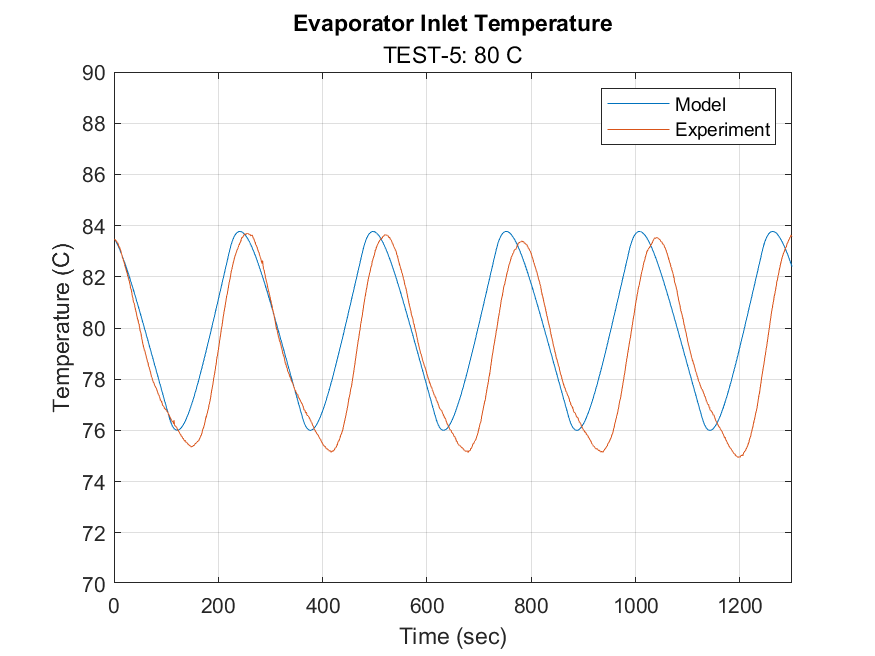
\includegraphics[width=7.2cm]{images/TEST-5.png}
        \captionof{figure}{Test-5.}
        \label{fig:test5}
    \end{minipage}%
    \begin{minipage}{.4\textwidth}
        \centering
        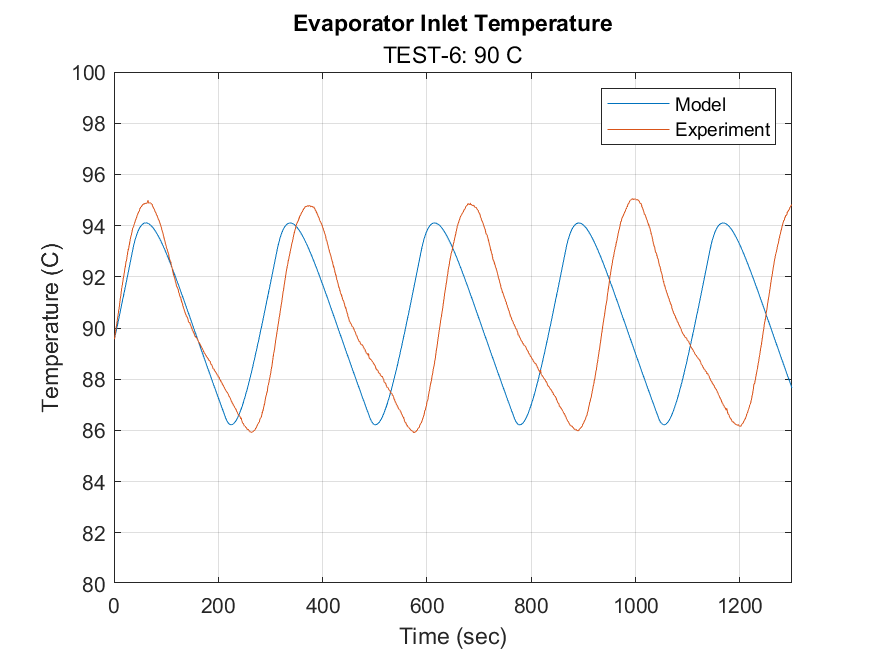
\includegraphics[width=7.2cm]{images/TEST-6.png}
        \captionof{figure}{Test-6.}
        \label{fig:test6}
    \end{minipage}
\end{figure}

\bigskip

\begin{figure}
    \centering
    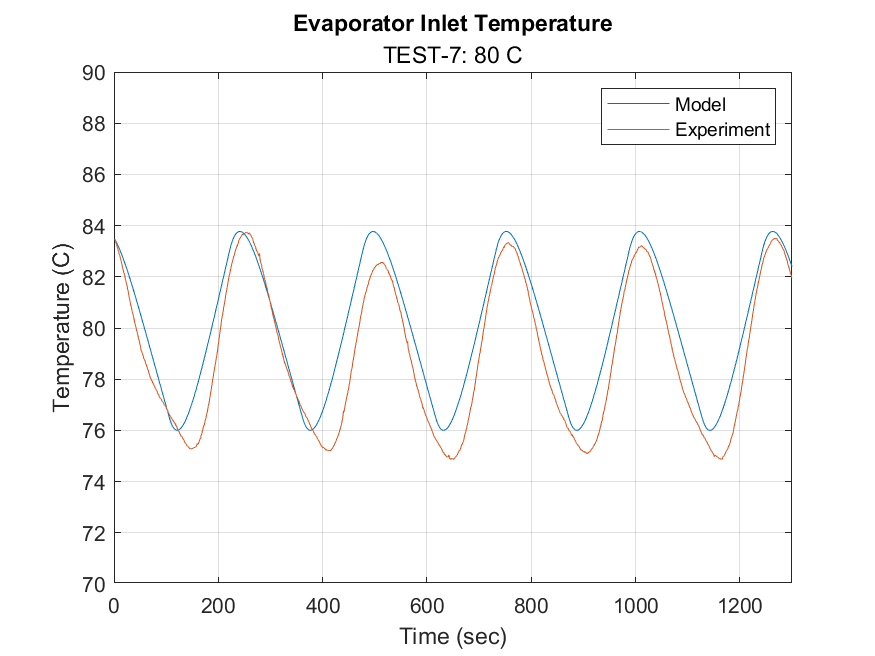
\includegraphics[width=7.2cm]{images/TEST-7.png}
    \caption{Test-7.}
    \label{fig:test7}
\end{figure}

As can be seen, the results of the simulations are highly coherent with the experiment results. Tests 3 and 7 show that the model produces better results at low set temperatures, except for test 5. Test 4 and 6 demonstrates that the model data has a slightly low period than the experiment data when the set temperature is high.

\section{Result of the Bypass Pipeline}

To see if the proposed solution works or not, the model is tested by setting a bypass rate. Then the results are compared with the older results without bypass line usage. The decrease in the oscillation amplitude is measured. The resulting plot is provided in Figure \ref{fig:result}.

\begin{figure}[H]
    \centering
    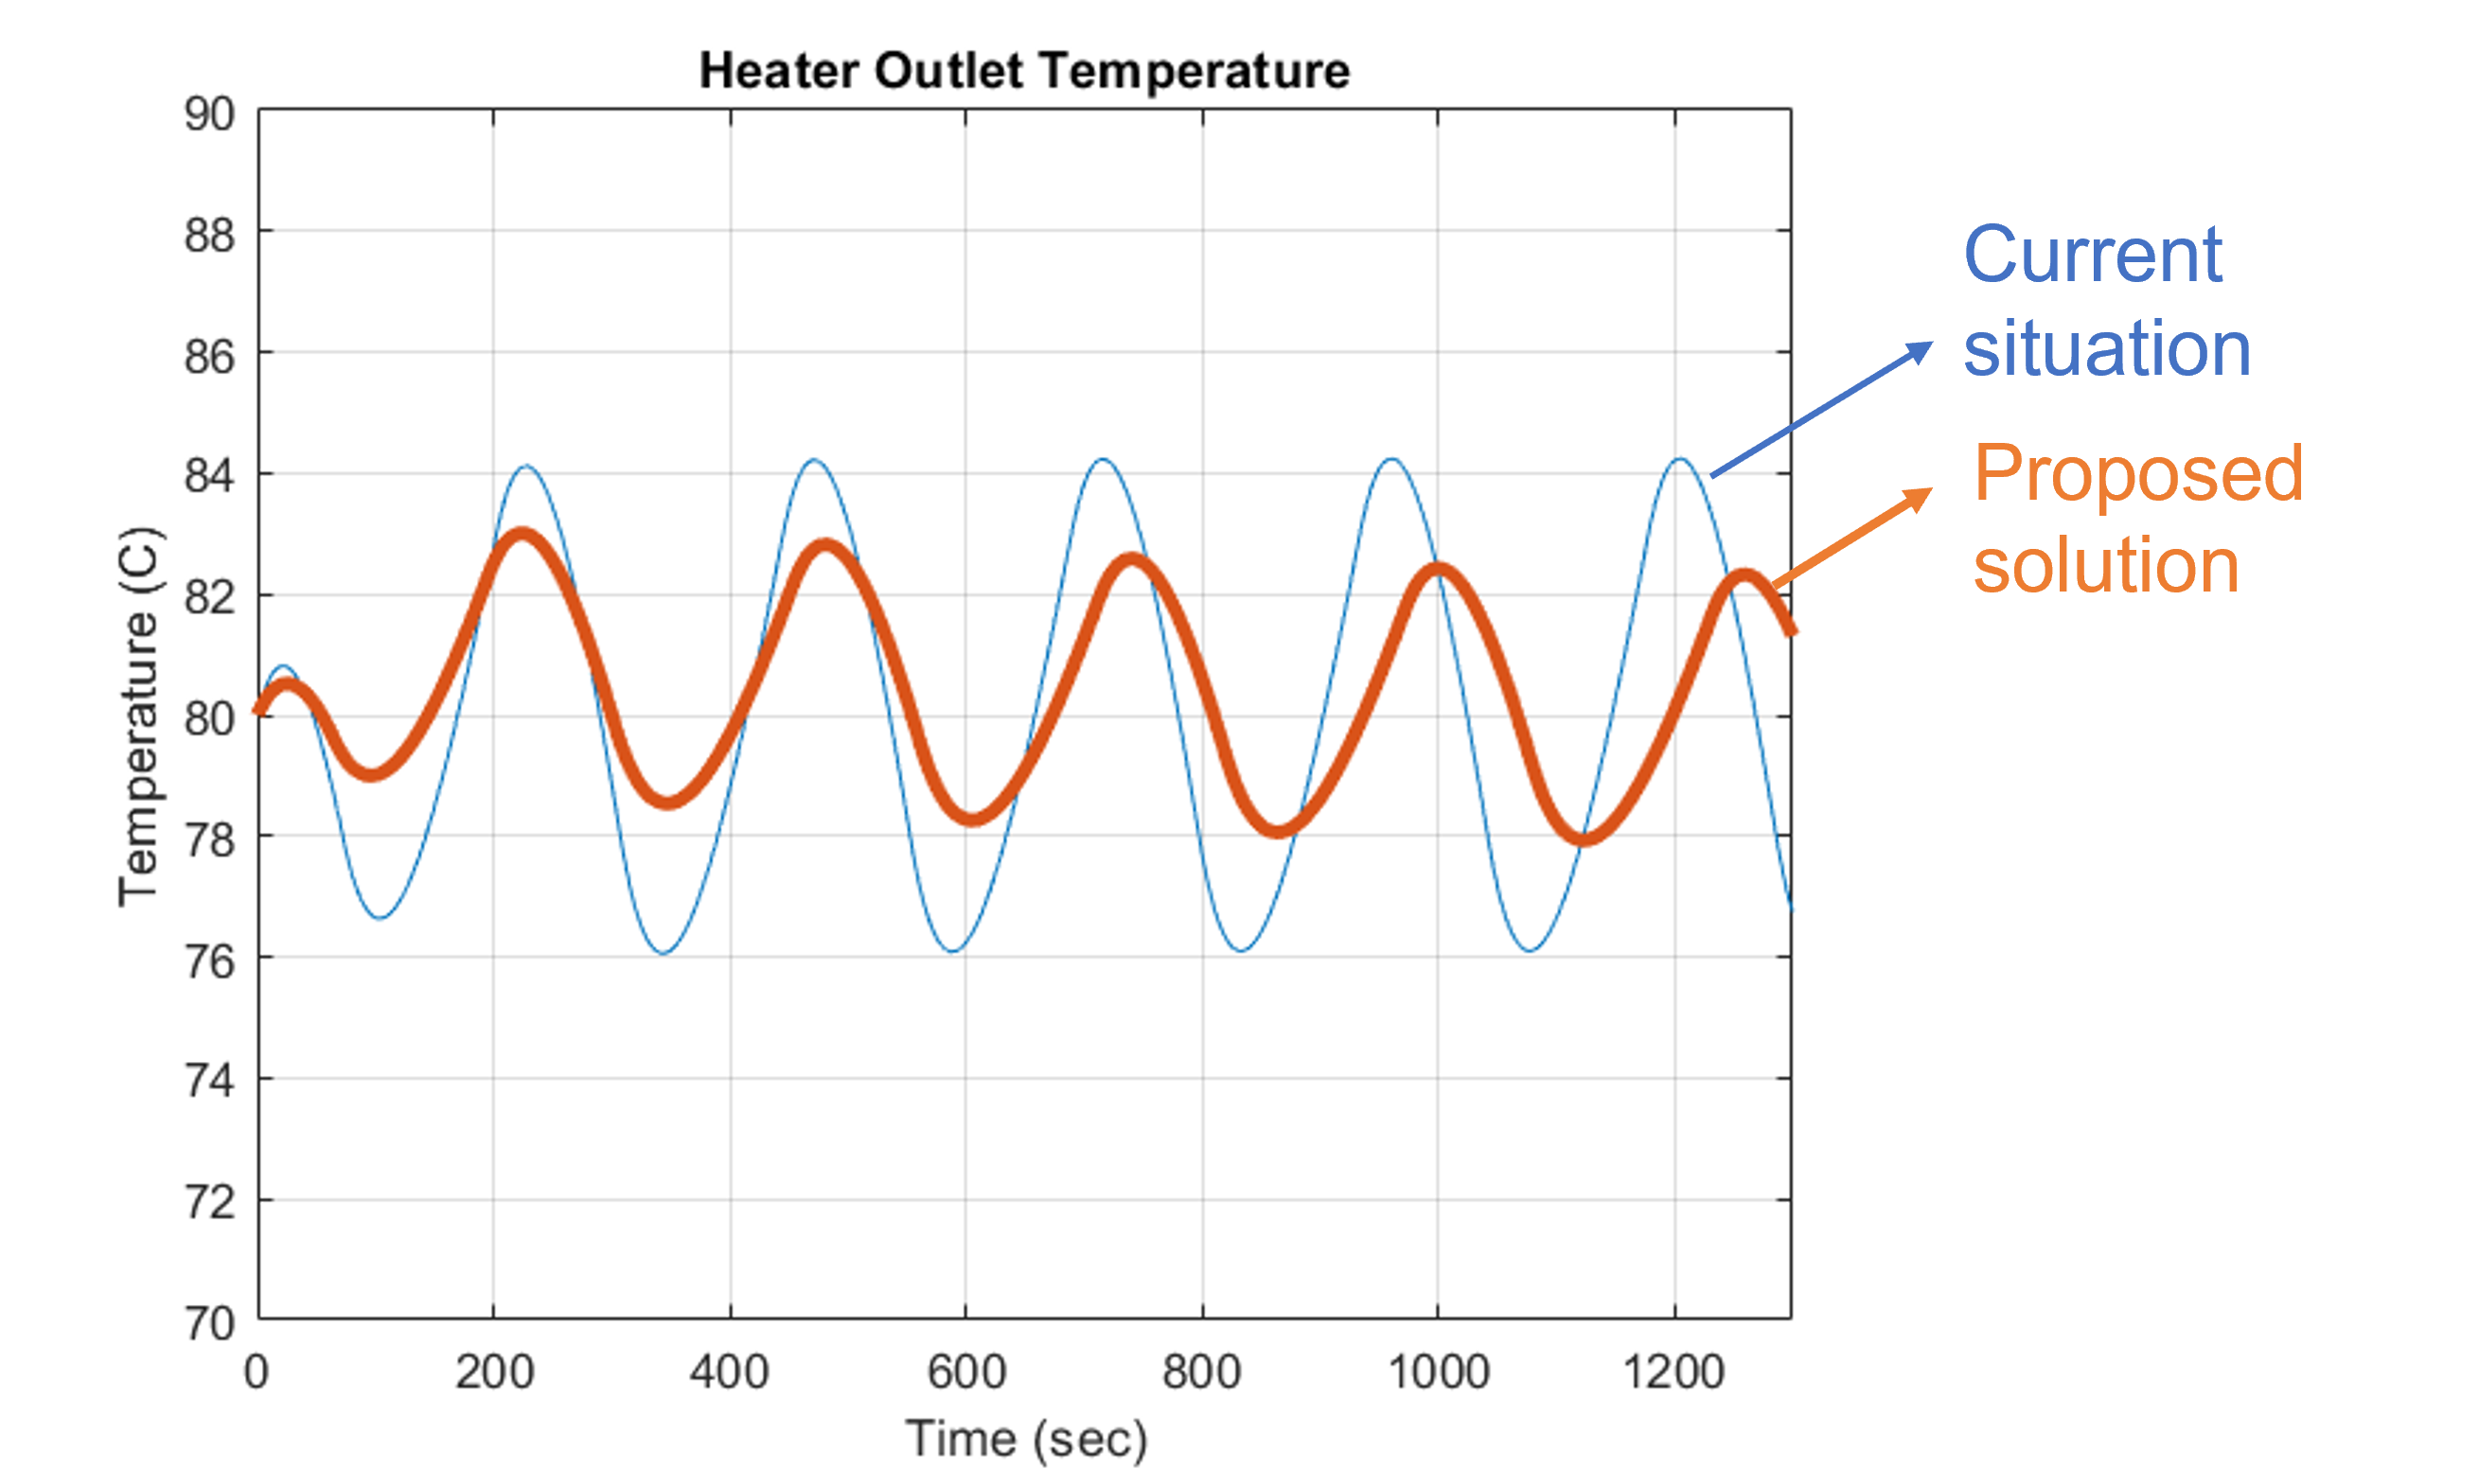
\includegraphics[width=12cm]{images/result.png}
    \caption{Comparison of temperature oscillation results with the solution.}
    \label{fig:result}
\end{figure}

As seen in Figure \ref{fig:result}, several things are changed in the system's time response. Firstly, the oscillation amplitude is decreased as expected. Furthermore, the oscillation period is increased, which has no effect on the cycle, either positive or negative. Thus, results are satisfactory in the sense of decreasing the oscillation magnitude.

\par
On the other hand, there are several things to be noted. When the bypass line is used, the set temperature needs to be set to a higher temperature. Also, the oil flowing in the cycle will be at higher temperatures to compensate for the temperature decrease in the evaporator inlet due to mixing with cooler oil. Higher temperatures overall can lead to more heat loss and, eventually, more power consumption. Additionally, higher temperatures in the components can increase material wearing. Lastly, the construction of this bypass system requires some amount of funding which should be taken into account as well.

\par
The system is tested at its limits to find out how much reduction can be maintained by specified bypass percentages and set temperatures. Two different tests are carried out by setting bypass rates of 50\% and 75\%. Results are provided in Tables \ref{tab:50} and \ref{tab:75}:

\begin{table}[h]
    \centering
    \begin{tabular}{|c c|}
        \hline
        Set temperature ($^\circ$C):   &  93 \\
        Bypass rate (\%):   &  50 \\
        Oscillation amplitude before ($^\circ$C):   &  7.0783 \\
        Oscillation amplitude after ($^\circ$C):   &  4.9918 \\
        Oscillation decrease percentage (\%):   &  30 \\
        \hline
    \end{tabular}
    \caption{Limits of the system when bypass rate is 50\%.}
    \label{tab:50}
\end{table}

\begin{table}[h]
    \centering
    \begin{tabular}{|c c|}
        \hline
        Set temperature ($^\circ$C):   &  120 \\
        Bypass rate (\%):   &  75 \\
        Oscillation amplitude before ($^\circ$C):   &  7.0783 \\
        Oscillation amplitude after ($^\circ$C):   &  3.0159 \\
        Oscillation decrease percentage (\%):   &  57 \\
        \hline
    \end{tabular}
    \caption{Limits of the system when bypass rate is 75\%.}
    \label{tab:75}
\end{table}

\par
As a result, it is seen that the maximum decrease in oscillations can be achieved by 57\% with the maximum operating temperature for 80 $^\circ$C and 75\% bypass rate. Thus, considering the drawbacks mentioned above, this reduction is seen as not sufficient enough to construct the real system. Still, this model can be used for other investigation purposes in the oil cycle. Furthermore, this modeling process can be a guideline for researchers who want to model a power cycle in Matlab/Simulink.   

